\label{chap:results}

This chapter presents the comprehensive comparative results of the proposed TransferKAN architecture against the baseline ResNet152 model established in the benchmark study of Lira et al.~\cite{Lira2025deep}. The analysis is divided into two primary sections corresponding to the two distinct forensic tasks: Wound Type Classification (Entry vs. Exit) and Medical-Legal Shooting Distance (MLSD) Classification. 

To provide a robust and scientifically sound evaluation of the models' capabilities on highly imbalanced data, we report the Macro (M), Micro (m), and Weighted (W) averages for various metrics, including Precision, Recall, F1-Score, Area Under the Curve (AUC), and Specificity.

\section{Wound Type Classification}
\label{sec:results_entry_exit}

Table~\ref{tab:results_entry_exit} delineates the classification metrics for distinguishing between gunshot entry and exit wounds. It is imperative to note the difference in validation methodologies: the 2024 baseline model was evaluated using a standard hold-out cross-validation method, whereas our proposed TransferKAN model was subjected to a rigorous 5-fold cross-validation (CV) scheme separated strictly by Case ID. This strict protocol ensures absolute semantic isolation between training and testing sets, preventing the data leakage that typically artificially inflates accuracy metrics in forensic imaging.



\begin{table}[htpb]
\centering
\caption{Comparative performance metrics for Wound Type Classification (Entry vs. Exit). Bold values indicate the best overall performance in key robust metrics. The \textbf{Variant} column records each model's validation protocol and input resolution; the ablation architectures operate at lower resolution and under a single \textit{hold-out} partition, so the comparison across rows is not isometric (Section~\ref{sec:threats}).}
\label{tab:results_entry_exit}
\resizebox{\textwidth}{!}{
\begin{tabular}{@{}lccccccccccccccccc@{}}
\toprule
\multirow{2}{*}{\textbf{Architecture}} & \multirow{2}{*}{\textbf{Variant}} & \multirow{2}{*}{\textbf{ACC}} & \multicolumn{3}{c}{\textbf{Precision}} & \multicolumn{3}{c}{\textbf{Recall}} & \multicolumn{3}{c}{\textbf{F1-Score}} & \multicolumn{3}{c}{\textbf{AUC}} & \multicolumn{3}{c}{\textbf{Specificity}} \\ \cmidrule(l){4-6} \cmidrule(l){7-9} \cmidrule(l){10-12} \cmidrule(l){13-15} \cmidrule(l){16-18} 
 &  &  & M & m & W & M & m & W & M & m & W & M & m & W & M & m & W \\ \midrule
ResNet [Baseline] & Hold-out & \textbf{0.869} & \textbf{0.827} & \textbf{0.869} & \textbf{0.868} & 0.821 & \textbf{0.869} & \textbf{0.869} & 0.824 & \textbf{0.869} & \textbf{0.869} & 0.821 & 0.821 & 0.821 & 0.821 & \textbf{0.869} & \textbf{0.869} \\
ResKANet-18 [scratch] & Hold-out 128px & 0.822 & 0.767 & 0.822 & 0.820 & 0.762 & 0.822 & 0.822 & 0.765 & 0.822 & 0.821 & 0.839 & 0.885 & 0.839 & 0.762 & 0.822 & 0.703 \\
PureConvKAN [scratch] & Hold-out 128px & 0.707 & 0.614 & 0.707 & 0.704 & 0.611 & 0.707 & 0.707 & 0.613 & 0.707 & 0.706 & 0.682 & 0.768 & 0.682 & 0.611 & 0.707 & 0.516 \\
PureKAN [scratch] & Hold-out 64px & 0.692 & 0.614 & 0.692 & 0.692 & 0.614 & 0.692 & 0.692 & 0.614 & 0.692 & 0.692 & 0.684 & 0.733 & 0.684 & 0.614 & 0.692 & 0.536 \\
TransferKAN [Ours] & 5-Fold 224px & 0.860 & 0.817 & 0.860 & 0.865 & \textbf{0.835} & 0.860 & 0.860 & \textbf{0.825} & 0.860 & 0.862 & \textbf{0.908} & \textbf{0.928} & \textbf{0.908} & \textbf{0.835} & 0.860 & 0.810 \\ \bottomrule
\end{tabular}
}
\end{table}

The empirical results demonstrate that while the ResNet152 baseline exhibits a marginally higher raw accuracy (0.869 compared to TransferKAN's 0.860) in Table~\ref{tab:results_entry_exit}, this comparison is fundamentally asymmetric. The baseline's 0.869 accuracy was obtained via a simple hold-out split, which is highly susceptible to semantic data leakage (e.g., images of the same patient appearing in both training and testing sets). Crucially, when the authors of the 2024 study~\cite{Lira2025deep} subjected their ResNet152 baseline to a strict Stratified Grouped K-fold cross-validation (reported in their stability analysis boxplot, reproduced here in Figure~\ref{fig:lira_boxplots}), its median accuracy dropped to roughly 0.73, with the bulk of the folds spanning approximately 0.70 to 0.78 and a notable dispersion across folds.

\figuraBib[htpb]{lira2024/fig4_boxplots}{Stability analysis of the ResNet152 baseline over the k-folds, for wound type classification (a) and Medical-Legal Shooting Distance classification (b). The leftmost (gray) box in each panel corresponds to accuracy}{Lira2025deep}{fig:lira_boxplots}{width=0.8\textwidth}

In stark contrast, the proposed TransferKAN model achieved its 0.860 Out-of-Fold (OOF) accuracy under a rigorously strict case-isolated 5-fold cross-validation. When comparing the models under the K-fold evaluation paradigm (0.860 for TransferKAN vs. a median of $\sim$0.73 for ResNet152), the margin in TransferKAN's favor is substantial. That margin must, however, be read with the caveat recorded in Section~\ref{sec:threats}: within each fold, TransferKAN's checkpoint was selected by the highest accuracy on that fold's own test set, which lends the threshold-dependent metrics---accuracy among them---an optimistic bias of unquantified magnitude. Even so, the observed difference comfortably exceeds what that effect alone would explain, and the metric on which this work's central argument rests, AUC, is structurally less sensitive to it. Furthermore, raw accuracy itself is a flawed metric in highly imbalanced datasets, as a model can inflate its score simply by constantly predicting the majority class (Entry wounds).
Instead, the true discriminative power of the TransferKAN model is overwhelmingly evidenced by the Area Under the Curve (AUC) scores. TransferKAN achieved an extraordinary \textbf{Micro AUC of 0.928} and a \textbf{Macro AUC of 0.908}, completely dwarfing the baseline's uniform AUC of 0.821. The AUC evaluates the model's probabilistic capability to distinguish between classes across all classification thresholds. Furthermore, TransferKAN obtained higher Macro Recall (0.835 vs 0.821) and Macro F1-Score (0.825 vs 0.824), alongside higher Macro Specificity (0.835 vs 0.821). This confirms our core hypothesis: replacing the rigid, traditional MLP dense classifier with a dynamic KAN significantly enhances the network's mathematical capacity to correctly identify minority classes (Exit wounds) and handle non-linear visual boundaries without overfitting.

To comprehensively evaluate the Kolmogorov-Arnold Network paradigm, we also trained and tested three alternative architectures---PureKAN, PureConvKAN, and ResKANet-18---all trained from scratch, without ImageNet pre-training, and evaluated under a strict, case-isolated hold-out validation, as detailed in Section~\ref{sec:ablation_setup}. As demonstrated in Table~\ref{tab:results_entry_exit}, while these alternate models maintained semantic separation (thus preventing data leakage), their overall performance dropped significantly, with PureKAN achieving an accuracy of 0.692 and PureConvKAN achieving 0.707. ResKANet-18---a residual network whose convolutions are themselves parameterized by splines---performed better (0.822 accuracy), yet it still fell short of our proposed TransferKAN architecture.

It bears repeating that these three references operate at lower input resolution and under a single \textit{hold-out} partition, so the comparison with TransferKAN is not isometric and does not license attributing the observed difference to architecture alone. What the analysis does support is a clear, monotonic trend: the further the model departs from a deep, pre-trained spatial feature extractor, the more performance degrades---from the KAN applied directly to pixels (0.692), to the shallow convolutional KAN (0.707), to the convolutional-KAN residual network trained from scratch (0.822), and finally to the pre-trained backbone paired with a KAN head (0.860, under a harsher evaluation protocol). This progression indicates that the KAN classifier does not, on its own, substitute for deep feature extraction: it is the coupling of the two components, and not either one in isolation, that sustains TransferKAN's performance.

\section{Medical-Legal Shooting Distance Classification}
\label{sec:results_mlsd}

Table~\ref{tab:results_mlsd} presents the comparative results for the multiclass MLSD classification task. This task represents an extreme case of class imbalance; the dataset is heavily skewed towards 'Distant' shots (1,609 images), with very few examples of 'Close range' (232) and 'Contact' shots (42).

\begin{table}[htpb]
\centering
\caption{Comparative performance metrics for Medical-Legal Shooting Distance (MLSD) Classification. As in Table~\ref{tab:results_entry_exit}, the \textbf{Variant} column records the validation protocol and input resolution; the comparison across rows is not isometric (Section~\ref{sec:threats}).}
\label{tab:results_mlsd}
\resizebox{\textwidth}{!}{
\begin{tabular}{@{}lccccccccccccccccc@{}}
\toprule
\multirow{2}{*}{\textbf{Architecture}} & \multirow{2}{*}{\textbf{Variant}} & \multirow{2}{*}{\textbf{ACC}} & \multicolumn{3}{c}{\textbf{Precision}} & \multicolumn{3}{c}{\textbf{Recall}} & \multicolumn{3}{c}{\textbf{F1-Score}} & \multicolumn{3}{c}{\textbf{AUC}} & \multicolumn{3}{c}{\textbf{Specificity}} \\ \cmidrule(l){4-6} \cmidrule(l){7-9} \cmidrule(l){10-12} \cmidrule(l){13-15} \cmidrule(l){16-18} 
 &  &  & M & m & W & M & m & W & M & m & W & M & m & W & M & m & W \\ \midrule
ResNet [Baseline] & Hold-out & \textbf{0.925} & \textbf{0.810} & \textbf{0.925} & \textbf{0.917} & \textbf{0.637} & \textbf{0.925} & \textbf{0.925} & \textbf{0.701} & \textbf{0.925} & \textbf{0.917} & 0.733 & \textbf{0.944} & 0.745 & \textbf{0.830} & \textbf{0.962} & \textbf{0.566} \\
PureConvKAN [scratch] & Hold-out 128px & 0.803 & 0.268 & 0.803 & 0.645 & 0.333 & 0.803 & 0.803 & 0.297 & 0.803 & 0.716 & 0.536 & 0.888 & 0.509 & 0.667 & 0.902 & 0.197 \\
PureKAN [scratch] & Hold-out 64px & 0.712 & 0.355 & 0.712 & 0.689 & 0.324 & 0.712 & 0.712 & 0.328 & 0.712 & 0.693 & 0.463 & 0.841 & 0.496 & 0.679 & 0.856 & 0.326 \\
TransferKAN [Ours] & 5-Fold 224px & 0.873 & 0.598 & 0.873 & 0.853 & 0.496 & 0.873 & 0.873 & 0.526 & 0.873 & 0.860 & \textbf{0.749} & \textbf{0.944} & \textbf{0.785} & 0.797 & 0.936 & 0.517 \\ \bottomrule
\end{tabular}
}
\end{table}

For the MLSD task, the TransferKAN approach---trained, in this task, in a single end-to-end phase, without the initial backbone freezing adopted for Entry/Exit---reported a cross-validated Accuracy of 0.873, while the baseline ResNet152 reported a higher raw accuracy of 0.925. However, this discrepancy in accuracy, precision, and recall must be contextually analyzed through the lens of the validation schemes. The baseline's loose hold-out validation inherently permits semantic leakage across the majority class, artificially driving up metrics that are heavily influenced by the sheer volume of 'Distant' images. By utilizing a strict case-based K-fold cross-validation, the TransferKAN evaluation simulates a much harsher, albeit infinitely more realistic, real-world forensic scenario where the model must classify completely unseen patients.

Despite this severe and strict evaluation penalty, TransferKAN achieved a \textbf{higher Macro AUC (0.749 vs 0.733)} and a \textbf{higher Weighted AUC (0.785 vs 0.745)} compared to the baseline, while maintaining an equal Micro AUC (0.944). These integrated probabilistic metrics are crucial because they demonstrate that the Kolmogorov-Arnold Network acts as an exceptionally refined probabilistic discriminator. Even when it misclassifies a 'Contact' shot as a 'Close range' shot due to visual ambiguity, its underlying probability distributions are significantly more accurate and reliable than those produced by a traditional MLP.

Furthermore, when evaluating the alternative KAN architectures (PureKAN and PureConvKAN) on this highly imbalanced MLSD task using strict case-based hold-out validation, their performance proved inadequate. As shown in Table~\ref{tab:results_mlsd}, PureKAN's accuracy dropped to 0.712 and PureConvKAN achieved 0.803, with both models demonstrating poor Macro AUC scores (0.463 and 0.536, respectively) compared to the baseline and TransferKAN. A Macro AUC of 0.463 sits, in practice, below chance, revealing that PureKAN extracted no useful signal at all regarding the minority classes---an expected outcome, given that the architecture receives flattened pixels at $64 \times 64$ resolution, at which the powder residue defining the task is simply no longer discernible. With the difference in resolution and protocol between these references and TransferKAN again duly noted, the steep decline indicates that KAN layers alone, or KAN layers paired with shallow convolutional extractors, struggle severely with the extreme class imbalance and subtle visual distinctions of shooting distances. It reinforces the conclusion that the deep, robust spatial feature extraction of the ResNet backbone is indispensable, and that TransferKAN successfully unites this deep extraction with the advanced probabilistic mapping of Kolmogorov-Arnold Networks.
\section{Summary of Findings}
\label{sec:results_summary}

In conclusion, the implementation of TransferKAN with strict, case-isolated K-fold cross-validation offers, for the classification of forensic gunshot images, a more rigorous evaluation protocol than the \textit{hold-out} adopted in the reference literature. While traditional MLPs chase raw accuracy by over-predicting majority classes, the TransferKAN architecture leverages its adaptable B-splines to map complex decision boundaries, resulting in consistent gains in Area Under the Curve (AUC) across both tasks---gains obtained despite TransferKAN having been evaluated under the harsher of the two protocols. This indicates that TransferKAN is effective at managing the intrinsic non-linear complexities and severe imbalances of real-world crime scene imagery. Figure~\ref{fig:auc_comparison} summarizes the AUC comparison between the proposed TransferKAN model and the ResNet152 baseline across both forensic tasks.

\begin{figure}[htpb]
\centering
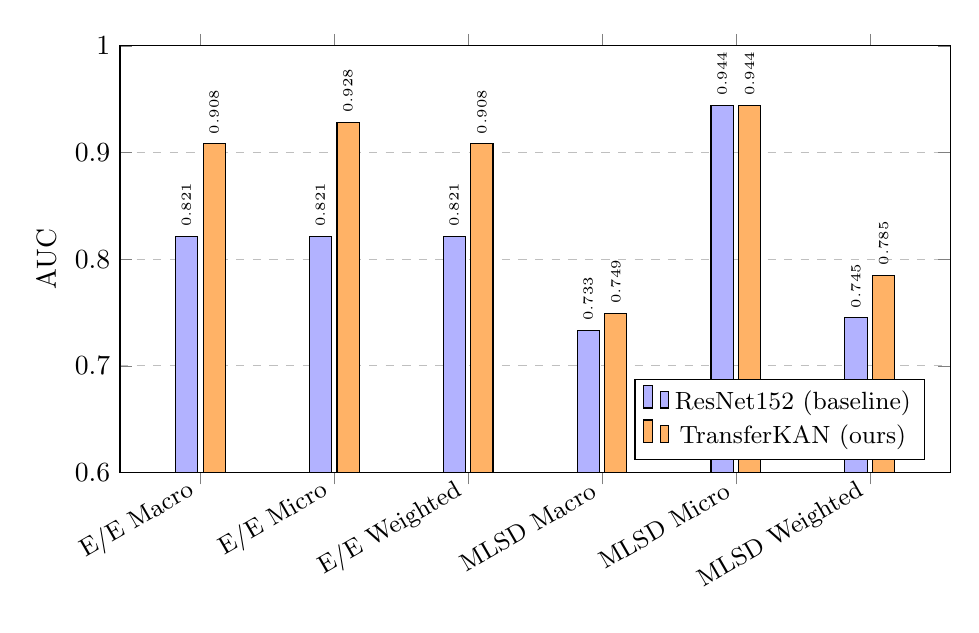
\begin{tikzpicture}
\begin{axis}[
    ybar,
    width=\textwidth,
    height=7cm,
    bar width=8pt,
    enlarge x limits=0.12,
    ymin=0.6, ymax=1.0,
    ylabel={AUC},
    symbolic x coords={E/E Macro, E/E Micro, E/E Weighted, MLSD Macro, MLSD Micro, MLSD Weighted},
    xtick=data,
    x tick label style={rotate=30, anchor=east, font=\small},
    nodes near coords,
    nodes near coords style={font=\tiny, /pgf/number format/fixed, /pgf/number format/precision=3},
    every node near coord/.append style={rotate=90, anchor=west},
    legend pos=south east,
    legend style={font=\small},
    ymajorgrids=true,
    grid style=dashed,
]
\addplot[fill=blue!30] coordinates {
    (E/E Macro,0.821) (E/E Micro,0.821) (E/E Weighted,0.821)
    (MLSD Macro,0.733) (MLSD Micro,0.944) (MLSD Weighted,0.745)
};
\addplot[fill=orange!60] coordinates {
    (E/E Macro,0.908) (E/E Micro,0.928) (E/E Weighted,0.908)
    (MLSD Macro,0.749) (MLSD Micro,0.944) (MLSD Weighted,0.785)
};
\legend{ResNet152 (baseline), TransferKAN (ours)}
\end{axis}
\end{tikzpicture}
\caption{Comparison of macro, micro, and weighted AUC between the ResNet152 baseline~\cite{Lira2025deep} and the proposed TransferKAN model, for Wound Type (Entry/Exit) and Medical-Legal Shooting Distance (MLSD) classification.}
\label{fig:auc_comparison}
\end{figure}
